%%=============================================================================
%% Methodologie
%%=============================================================================

\chapter{\IfLanguageName{dutch}{Methodologie}{Methodology}}%
\label{ch:methodologie}

\begin{figure*}[h]
    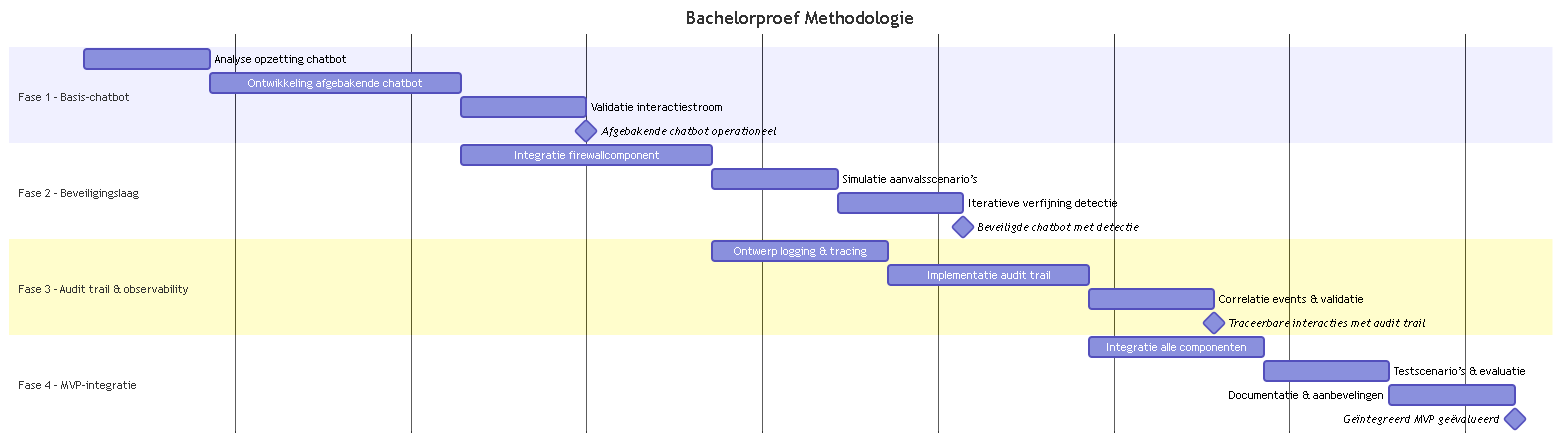
\includegraphics[width=\textwidth]{gantt.png}
    \caption{Gantt-diagram}
\end{figure*}

\noindent Dit onderzoek wordt uitgevoerd als toegepast onderzoek binnen de bedrijfscontext van Evolane en focust op één afgebakende probleemsituatie, namelijk het gebrek aan traceerbaarheid en beveiliging van AI-gestuurde chatbotinteracties binnen klantondersteuningsprocessen. Het onderzoek resulteert in een minimum viable product (MVP), zijnde een eerste functionele implementatie waarin de kernfunctionaliteiten voor traceerbaarheid en beveiliging aantoonbaar aanwezig zijn. De scope van het onderzoek beperkt zich tot het technisch ontwerpen, implementeren en evalueren van dit prototype binnen een gecontroleerde testomgeving.\\

\noindent Het proof-of-concept wordt opgebouwd in vier opeenvolgende, inhoudelijk samenhangende fasen. Elke fase levert een concrete mijlpaal op die bijdraagt aan het beantwoorden van de centrale onderzoeksvraag.

\paragraph{Fase 1: Ontwikkeling van een afgebakende chatbot}
In de eerste fase wordt een eenvoudige chatbot ontwikkeld die één concreet klantondersteuningsscenario implementeert. De functionaliteit blijft bewust beperkt tot een duidelijk afgelijnde use case, zodat de interactiestroom tussen gebruiker en digitale assistent reproduceerbaar blijft. De chatbot dient uitsluitend als testobject voor verdere beveiligings- en traceerbaarheidsmechanismen. Het eindresultaat van deze fase is een functionerende chatbot met een stabiele interactiestroom.

\paragraph{Fase 2: AI firewall voor chatbotverkeer}
In de tweede fase wordt het chatbotverkeer voorzien van een beveiligingslaag die inkomende en uitgaande interacties analyseert. De focus ligt op het detecteren en blokkeren van afwijkende of risicovolle invoer binnen de afgebakende testomgeving. Door het uitvoeren van gesimuleerde aanvalsscenario’s wordt nagegaan hoe effectief het systeem reageert op misbruik van de chatbotinterface. Deze fase resulteert in een chatbot waarbij beveiligingsdetectie en -mitigatie functioneren.

\paragraph{Fase 3: Implementatie van traceerbaarheid en audit trail}
De derde fase richt zich op het vastleggen en overeenkomen van gebeurtenissen binnen de chatbotinteracties. Hierbij worden gebruikersacties, systeemreacties en beveiligingsgebeurtenissen gelogd om volledige reconstructie van gesprekken mogelijk te maken. De audit trail wordt opgezet met als doel technische reproduceerbaarheid van incidenten, zonder dat juridische bewijsvoering of langdurige datastorage wordt nagestreefd. Het eindresultaat van deze fase is een werkende audit trail die inzicht biedt in het volledige verloop van interacties.

\paragraph{Fase 4: Integratie en evaluatie van het MVP}
In de vierde fase worden alle ontwikkelde componenten samengebracht tot één geïntegreerd MVP. Dit prototype wordt geëvalueerd aan de hand van vooraf gedefinieerde testscenario’s die zowel normale interacties als afwijkend gedrag omvatten. De evaluatie focust op de mate waarin het systeem traceerbaarheid en beveiliging combineert binnen de afgebakende casus. Deze fase resulteert in een geïntegreerd MVP en een technische evaluatie die de basis vormt voor aanbevelingen.

